\section{Berkeley Case: No Latent Confounding}\label{sec:modeling}
 % \begin{figure}[ht]
%      \centering
%      \begin{subfigure}{0.9\linewidth}
%      \centering
%             \begin{tikzpicture}
%             \tikzstyle{vertex}=[circle,fill=none,draw=black,minimum size=17pt,inner sep=0pt]
% \node[vertex] (S) at (0,0) {$S$};
% \node[vertex] (A) at (2,0) {$A$};
% \node[vertex] (D) at (1,1) {$D$};
% \path (S) edge (D);
% \path (D) edge (A);
% \path[red] (S) edge (A);
%             \end{tikzpicture}
%         \caption{Causal graph for $\model \in \modelsunconfedge$ illustrating all possible functional dependencies.}
%         \label{fig:no-cf-edge}
%         \end{subfigure}    \hfill
% %              \begin{subfigure}{0.45\linewidth}
% %              \centering
% %             \begin{tikzpicture}
% %             \tikzstyle{vertex}=[circle,fill=none,draw=black,minimum size=17pt,inner sep=0pt]
% % \node[vertex] (S) at (0,0) {$S$};
% % \node[vertex] (A) at (2,0) {$A$};
% % \node[vertex] (D) at (1,1) {$D$};
% % \path (S) edge (D);
% % \path (D) edge (A);
% % %\path[red] (S) edge (A);
% %             \end{tikzpicture}
% %         \caption{Causal graph for $\model \in \nullgraphunconf$ illustrating all possible functional dependencies.}
% %         \label{fig:no-cf-no-edge}
% %         \end{subfigure}
% \end{figure}

% \begin{figure}[h]
%      \centering
%             \begin{tikzpicture}
%             \tikzstyle{vertex}=[circle,fill=none,draw=black,minimum size=17pt,inner sep=0pt]
% \node[vertex] (S) at (0,0) {$S$};
% \node[vertex] (A) at (2,0) {$A$};
% \node[vertex] (D) at (1,1) {$D$};
% \path (S) edge (D);
% \path (D) edge (A);
% \path[bidirected] (D) edge[bend left=60] (A);
% \path[red] (S) edge (A);
% % \draw[->, line width=0.3mm]  (S)--(D);
% % \draw[->, line width=0.3mm]  (D)--(A);
% % \draw[->, line width=0.3mm]  (S)--(A);
% % \draw[<->, line width=0.3mm]  (D)--(A);
%             \end{tikzpicture}
%         \caption{Causal graph for $\model \in \modelsunconfedge$ illustrating all possible functional dependencies.}
%         \label{fig:cf-no-edge}
% \end{figure}

% \begin{figure}[h]
%      \centering
%             \begin{tikzpicture}
%             \tikzstyle{vertex}=[circle,fill=none,draw=black,minimum size=17pt,inner sep=0pt]
% \node[vertex] (S) at (0,0) {$S$};
% \node[vertex] (A) at (3,-0.5) {$A$};
% \node[vertex] (D) at (1,1) {$D$};
% \node[vertex] (S') at (1,-0.5) {$S'$};
% \path (S) edge (D);
% \path (D) edge (A);
% \path[bidirected] (D) edge[bend left=60] (A);
% \path[red] (S') edge (A);
% %\path (S) edge (S'); 
%  \path (S) edge node[near start, below] {=} (S');
% % \draw[->, line width=0.3mm]  (S)--(D);
% % \draw[->, line width=0.3mm]  (D)--(A);
% % \draw[->, line width=0.3mm]  (S)--(A);
% % \draw[<->, line width=0.3mm]  (D)--(A);
%             \end{tikzpicture}
%         \caption{Causal graph for $\model \in \modelsedge$ illustrating all possible functional dependencies.} 
%         \label{fig:cf-edge}
% \end{figure}


%              \begin{subfigure}{0.45\linewidth}
%              \centering
%             \begin{tikzpicture}
%             \tikzstyle{vertex}=[circle,fill=none,draw=black,minimum size=17pt,inner sep=0pt]
% \node[vertex] (S) at (0,0) {$S$};
% \node[vertex] (A) at (2,0) {$A$};
% \node[vertex] (D) at (1,1) {$D$};
% \path (S) edge (D);
% \path (D) edge (A);
% %\path[red] (S) edge (A);
%             \end{tikzpicture}
%         \caption{Causal graph for $\model \in \nullgraphunconf$ illustrating all possible functional dependencies.}
%         \label{fig:no-cf-no-edge}
%         \end{subfigure}
%\end{figure}

\begin{figure*}[t]
     \centering
     \begin{subfigure}{0.32\linewidth}
     \centering
            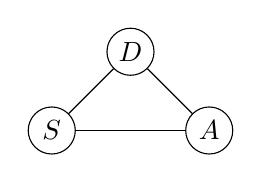
\begin{tikzpicture}
            \tikzstyle{vertex}=[circle,fill=none,draw=black,minimum size=17pt,inner sep=0pt]
\node[vertex] (S) at (0,0) {$S$};
\node[vertex] (A) at (2,0) {$A$};
\node[vertex] (D) at (1,1) {$D$};
\path (S) edge (D);
\path (D) edge (A);
\path (S) edge (A);
            \end{tikzpicture}
        \caption{$\model \in \modelsunconfedge$}
        \label{fig:no-cf-edge}
\end{subfigure}
     \begin{subfigure}{0.32\linewidth}
     \centering
            \begin{tikzpicture}
            \tikzstyle{vertex}=[circle,fill=none,draw=black,minimum size=17pt,inner sep=0pt]
\node[vertex] (S) at (0,0) {$S$};
\node[vertex] (A) at (2,0) {$A$};
\node[vertex] (D) at (1,1) {$D$};
%\node[vertex] (S') at (1,-0.5) {$S'$};
\path (S) edge (D);
\path (D) edge (A);
\path[bidirected] (D) edge[bend left=60] (A);
\path (S) edge (A);
%\path (S) edge (S'); 
% \path (S) edge node[near start, below] {=} (S');
% \draw[->, line width=0.3mm]  (S)--(D);
% \draw[->, line width=0.3mm]  (D)--(A);
% \draw[->, line width=0.3mm]  (S)--(A);
% \draw[<->, line width=0.3mm]  (D)--(A);
            \end{tikzpicture}
        \caption{$\model \in \modelsedgerelax$} 
        \label{fig:cf-edge}
        \end{subfigure}
         \begin{subfigure}{0.32\linewidth}
     \centering
            \begin{tikzpicture}
            \tikzstyle{vertex}=[circle,fill=none,draw=black,minimum size=17pt,inner sep=0pt]
\node[vertex] (S) at (0,0) {$S$};
\node[vertex] (A) at (2,0) {$A$};
\node[vertex] (D) at (1,1) {$D$};
%\node[vertex] (S') at (1,-0.5) {$S'$};
\path (S) edge (D);
\path (D) edge (A);
\path[bidirected] (D) edge[bend left=60] (A);
%\path (S) edge (A);
%\path (S) edge (S'); 
% \path (S) edge node[near start, below] {=} (S');
% \draw[->, line width=0.3mm]  (S)--(D);
% \draw[->, line width=0.3mm]  (D)--(A);
% \draw[->, line width=0.3mm]  (S)--(A);
% \draw[<->, line width=0.3mm]  (D)--(A);
            \end{tikzpicture}
        \caption{$\model \in \nullgraph$ and $\model \in \modeliv$} 
        \label{fig:cf-edge-iv}
        \end{subfigure}
        \caption{Causal graphs, $\cg{\model}$, assumed in various model classes.}
\end{figure*}

% \begin{figure}
%      \centering
%             \begin{tikzpicture}
%             \tikzstyle{vertex}=[circle,fill=none,draw=black,minimum size=17pt,inner sep=0pt]
% \node[vertex] (Z) at (0,0) {$Z$};
% \node[vertex] (Y) at (3,0) {$Y$};
% \node[vertex] (X) at (1.5,0) {$X$};
% %\node[vertex] (S') at (1,-0.5) {$S'$};
% \path (Z) edge (X);
% \path (X) edge (Y);
% \path[bidirected] (X) edge[bend left=60] (Y);
% %\path[red] (S') edge (A);
% %\path (S) edge (S'); 
%  %\path (S) edge node[near start, below] {=} (S');
% % \draw[->, line width=0.3mm]  (S)--(D);
% % \draw[->, line width=0.3mm]  (D)--(A);
% % \draw[->, line width=0.3mm]  (S)--(A);
% % \draw[<->, line width=0.3mm]  (D)--(A);
%             \end{tikzpicture}
%         \caption{Causal graph of $M \in \modeliv$} 
%         \label{fig:iv}
%         \end{figure}

Under the semantic framework of SCMs, we first make the same causal modeling assumptions that are commonplace in works that mention the Berkeley admissions case. We compare fairness notions that are tied to these modeling assumptions, with the view that modeling assumptions describe a family of SCMs and fairness notions define a subset of this family. We relate existing general notions of fairness in the literature to this viewpoint. While this is a re-examination of the various existing analyses of the Berkeley admissions case, in the next section, we relax the causal modeling assumptions and consider the more general family of models that allow for confounding between department choice and admissions outcome.

The set of endogenous variables consists of the protected attribute, namely sex of the applicant, $\sex$, the department they applied to, $\dept$, and the decision of the admissions committee, $\outcome$. We assume that $\sex, \outcome$ are binary variables and $\dept$ is a discrete-valued variable taking finite number of values, where $\sex=0,1$ corresponds to male, female applicants, respectively, and $\outcome=0,1$ corresponds to reject and accept, respectively.\footnote{The assumption of binary sex is purely for mathematical simplicity.} Given that, possibly, societal biases nudge applicants to departments at differing rates depending on their sex, we assume that $\sex$ affects $\dept$. Since departments are the primary decision-making units and have different admission rates, we also assume that $\dept$ affects $\outcome$. The question of whether acceptance decisions discriminate against sex centers around the direct causal effect of $\sex$ on $\outcome$, and therefore we allow such an effect in the model. We assume the absence of any confounding between the variables (in addition to the absence of any selection bias). The structural equations are given by
\ifdefined\SINGLE
\begin{align}\label{eq:no-cf-edge}
    \sex &= f_{\sex}(U_{\sex}) \nonumber, \\
    \dept &= f_{\dept}(\sex, U_{\dept}), \\
    \outcome &= f_{\outcome}(\sex,\dept,U_{\outcome}), \nonumber
\end{align}
\else $\sex = f_{\sex}(U_{\sex}), 
    \dept = f_{\dept}(\sex, U_{\dept}),
    \outcome = f_{\outcome}(\sex,\dept,U_{\outcome})$
\fi 
where $U_{\sex},U_{\dept}$ and $U_{\outcome}$ denote independent exogenous random variables. We denote the family of SCMs parameterized by the \ifdefined\SINGLE functions in \eqref{eq:no-cf-edge} \else above functions\fi and the exogenous distribution as $\modelsunconfedge$. 
%Let $\modelsunconfnoedge$ represent the same but where $\sex$ does not affect $\outcome$. 
For $\model \in \modelsunconfedge$, the causal graph $G(\model)$ is a directed acyclic graph (DAG), a subgraph of the one in Figure~\ref{fig:no-cf-edge}. 

\subsection{Fairness Notions}
We define a fairness notion to be a certain condition that is required to be satisfied by a causal model to be deemed fair. These conditions can take the form of observational, interventional, counterfactual or graphical queries on the SCMs in the families of causal models defined by modeling assumptions, in our case, $\modelsunconfedge$. While the criteria for the fairness notions in Section~\ref{sec:modeling} are phrased in terms of queries corresponding to different rungs of the causal ladder, in our case, any condition can only be tested using observational data.

% \ifdefined\SINGLE
% \begin{definition}[Demographic Parity]
% $\model \in \modelsunconfedge$ is fair according to demographic parity if it belongs to the null hypothesis set $\nullobsunconf \triangleq \left \lbrace \model \in \modelsunconfedge : P_{\model}\Paren{\outcome=1 \mid \sex =0} = P_{\model}\Paren{\outcome=1 \mid \sex=1} \right \rbrace $.
% \end{definition}
% \else
% \begin{definition}[Observational Notion of Fairness]
% $\model \in \modelsunconfedge$ is fair according to the observational notion of fairness if it belongs to 
% \begin{align*}
% \nullobsunconf &\triangleq \left \lbrace \model \in \modelsunconfedge : \right.\\
% &\left. P_{\model}\Paren{\outcome=1 \mid \sex =0} = P_{\model}\Paren{\outcome=1 \mid \sex=1} \right \rbrace.
% \end{align*}
% \end{definition}
% \fi

% The observational notion of fairness defined above is termed demographic parity \citep{DworkHPRZ12} in modern-day fairness literature and has implicitly been mentioned in earlier works \citep{HutchinsonMitchell19}. This is the notion of fairness that prompted the investigation of \cite{BickelHO75} into the Berkeley admissions data. We have already mentioned that this fairness notion falls prey to Simpson's paradox, i.e. Simpson's paradox translates into a fairness paradox where aggregated over the departments, the decision-making is unfair whereas for each department separately, it is fair. 

% We now mention another observational notion of fairness that is similar to a conditional version of demographic parity. 

The investigation of Berkeley's admission data was initiated on the observation that the well-known fairness notion of demographic parity $P_{\model}\Paren{\outcome=1 \mid \sex = 0} = P_{\model}\Paren{\outcome=1 \mid \sex = 1}$ did not hold. This fairness notion is based purely on observational data and we have already noted that it falls prey to Simpson's paradox. We now present another observational notion of fairness that can be interpreted as a conditional version of demographic parity.
\ifdefined\SINGLE
\begin{definition}[Observational Notion of Fairness]
$\model \in \modelsunconfedge$ is fair according to the observational notion of fairness if it belongs to the null hypothesis set 
\begin{align*}
\nullobsunconf \triangleq &\left \lbrace \model \in \modelsunconfedge :  \forall \ldept, \lsex, P_{\model}\Paren{\dept = \ldept, \sex = \lsex} >0 \right.\\
&\left. \implies P_{\model}\Paren{\outcome=1 \mid \sex =\lsex, \dept = \ldept} = P_{\model}\Paren{\outcome=1 \mid \dept = \ldept} \right \rbrace.
\end{align*}
% $$\nullobsunconf \triangleq \left \lbrace \model \in \modelsunconfedge : \forall \ldept, \lsex: P_{\model}\Paren{\dept = \ldept, \sex = \lsex} >0,  P_{\model}\Paren{\outcome=1 \mid \sex =\lsex, \dept = \ldept} = P_{\model}\Paren{\outcome=1 \mid \dept = \ldept} \right \rbrace. $$
\end{definition}
\else
\begin{definition}[Observational Notion of Fairness]
$\model \in \modelsunconfedge$ is fair according to the observational notion of fairness if it belongs to 
\begin{align*}
&\nullobsunconf \triangleq \left \lbrace \model \in \modelsunconfedge :  \forall \ldept, \lsex,  P_{\model}\Paren{\dept = \ldept, \sex = \lsex} >0 \right.\\
&\left. \implies P_{\model}\Paren{\outcome=1 \mid \sex =\lsex, \dept = \ldept} \right. \\
&\left.= P_{\model}\Paren{\outcome=1 \mid \dept = \ldept} \right \rbrace.
\end{align*}
\end{definition}
\fi

\citet{BickelHO75} proposed this notion for the Berkeley data. A valid test for this notion is a conditional independence test for $\outcome \indep \sex \mid \dept$. Indeed, the analysis of \citet{BickelHO75} shows that the data contain not enough evidence to reject the null hypothesis that this conditional independence holds, and therefore, concludes fairness. 

% \renewcommand{\thedefinition}{\thesection.\arabic{definition}} 
From the causal graph of $\modelsunconfedge$ in Figure~\ref{fig:no-cf-edge}, a natural subset of fair causal models is those without the edge $\sex \rightarrow \outcome$. 

\begin{definition}[Graphical Notion of Fairness]\label{def:graph_fairness}
     $\model \in \modelsunconfedge$ is fair according to the graphical notion of fairness if it belongs to the null hypothesis set $\nullgraphunconf \triangleq \left \lbrace \model \in \modelsunconfedge : \sex \rightarrow \outcome \notin \cg{\model} \right \rbrace$.
\end{definition}

% $\model \in \nullgraphunconf$ imposes a conditional independence constraint on the observational distribution, namely $\sex \indep \outcome \mid \dept$ by the global Markov property. Therefore, \citet{BickelHO75}'s analysis can be thought of as a valid test for the graphical notion of fairness albeit with an implicit faithfulness assumption.

\citet[Section 4.5.3]{Pearl09} discusses the direct effect in the context of the Berkeley admissions example, where he objects to conditioning for the department and instead proposes intervening on department choice, which corresponds to the controlled direct effect (CDE) \citep{Pearl01} of the `treatment', $\sex$, on the outcome, $\outcome$, for every value of the mediator, i.e., every department choice $\ldept$. 

\ifdefined\SINGLE
\begin{definition}[Interventional Notion of Fairness]
    $\model \in \modelsunconfedge$ is fair according to the interventional notion of fairness if it belongs to 
     \begin{equation*}\label{eq:interfairunconf}
    \nullinterunconf \triangleq \left \lbrace \model \in \modelsunconfedge: \forall \ldept,\lsex, P_{\model}\Paren{\outcome=1\mid\doop{\sex=\lsex},\doop{\dept=\ldept}} = P_{\model}\Paren{\outcome=1\mid\doop{\dept = \ldept}} \right \rbrace.
    \end{equation*}
    \end{definition}
\else
\begin{definition}[Interventional Notion of Fairness]
    $\model \in \modelsunconfedge$ is fair according to the interventional notion of fairness if it belongs to the null hypothesis set 
     \begin{align*}\label{eq:interfairunconf}
    &\nullinterunconf \triangleq \left \lbrace \model \in \modelsunconfedge: \forall \ldept,\lsex \right. \nonumber\\
   & \left. P_{\model}\Paren{\outcome=1\mid\doop{\sex=\lsex},\doop{\dept=\ldept}} \right. \nonumber\\
   &\left. = P_{\model}\Paren{\outcome=1\mid\doop{\dept = \ldept}} \right \rbrace.
    \end{align*}
\end{definition}
\fi
 % Note that, for the Berkeley example, a valid test for the interventional notion of fairness is again the conditional independence test $\outcome \indep \sex \mid \dept$.\footnote{This can be seen by applying the do-calculus and holds under positivity assumptions, which are met by the data at hand.}

Recent analyses of the Berkeley example emphasize counterfactual notions of fairness. In \citet[Section 4.5.4]{Pearl09}, \citet{PearlMackenzie18}, Pearl considers a counterfactual quantity, namely the natural direct effect (NDE) \citep{RobinsG92, Pearl01}  by motivating a hypothetical experiment where ``all female candidates retain their department preferences but change their gender [sex] identification (on the application form) from female to male''. Subsequent causal fairness works \citep{NabiShpitser18, Chiappa19} build on this and propose fairness notions based on known path-specific versions of NDE where the `direct path' from $\sex$ to $\outcome$ is viewed as `unfair' as opposed to the `fair' path $\sex \rightarrow \dept \rightarrow \outcome$. For the Berkeley example, the NDE$(s' \rightarrow s)$ is given by 
\begin{equation*}
P_{\model}\Paren{\outcome^{\doop{\sex = \lsex', \dept = \dept^{\doop{\sex=\lsex}}}}=1} - P_{\model}\Paren{\outcome^{\doop{\sex=s}}=1}
\end{equation*}
for $\lsex \neq \lsex'$. Note that by Pearl's mediation formula \citep{Pearl01}, the above is identified (assuming $\forall \ldept, \lsex, P_{\model}\Paren{\dept = \ldept, \sex = \lsex} > 0$) as 
\ifdefined\SINGLE
\begin{equation*}
    \sum\limits_{\ldept} \left( P_{\model}\Paren{\outcome=1 \mid \dept = \ldept, \sex = \lsex}  - P_{\model}\Paren{\outcome=1 \mid \dept = \ldept, \sex = \lsex'}\right)P_{\model}\Paren{\dept = \ldept \mid \sex= \lsex}.
\end{equation*}
\else
\begin{align*}
    \sum\limits_{\ldept} & \left( P_{\model}\Paren{\outcome=1 \mid \dept = \ldept, \sex = \lsex} \right. \\
    &\left. - P_{\model}\Paren{\outcome=1 \mid \dept = \ldept, \sex = \lsex'}\right)P_{\model}\Paren{\dept = \ldept \mid \sex= \lsex}.
\end{align*}
\fi
This implies that if the observational notion of fairness and positivity hold, the NDE is $0$. However, the converse is not necessarily true. For example, if one department favors male applicants and another favors female applicants, then the NDE could be $0$ while it is not necessary that the observational notion of fairness holds. 

Other counterfactual notions of fairness include those by \citet{KusnerLRS17}. The authors define a counterfactual fairness notion that implies demographic parity (see Section~\ref{app:kusnerctrfdemo} for a proof) for the Berkeley example; we have already seen that this particular fairness notion falls prey to Simpson's paradox. In the appendix, however, they define a path-dependent notion of counterfactual fairness.\footnote{This notion is specifically motivated by the Berkeley example.} In Section~\ref{app:kusnerpathnocf} we show that, in our setting, testing for the path-dependent counterfactual fairness notion is equivalent to testing for the conditional independence $A \indep S \mid D$. We now propose an alternate counterfactual notion of fairness and later compare testing of the same.
% Both the above notions correspond to not having a direct effect of $\sex$ on $\outcome$. Due to space constraints, we show the equivalence in supplementary material.

%that demands the invariance of the distribution of a decision, in a given context, with respect to a forced change in the protected attribute. 

\begin{definition}[Counterfactual Notion of Fairness]\label{def:ctrf-nocf}
$\model \in \modelsunconfedge$ is fair according to the counterfactual notion of fairness if it belongs to the null hypothesis set
\ifdefined\SINGLE
\begin{equation*}\label{eq:nullctrf}
    \nullctrfunconf \triangleq \left \lbrace \model \in \modelsunconfedge: \forall \ldept, \lsex, P_M(A^{\doop{S=s,D=d}} = A^{\doop{D=d}}) = 1 \right \rbrace.
\end{equation*}
\else
\begin{align*}\label{eq:nullctrf}
    \nullctrfunconf &\triangleq \left \lbrace \model \in \modelsunconfedge:\forall \ldept, \lsex,  \right. \nonumber\\
    &\left. P_M(A^{\doop{S=s,D=d}} = A^{\doop{D=d}}) = 1 \right \rbrace
\end{align*}
\fi
\end{definition}
The alternate hypotheses are given by the complement of the null hypotheses w.r.t. $\modelsunconfedge$. Given that the notions are defined on different rungs of the causal hierarchy, it is perhaps not surprising that they are nested accordingly. The assumption of no confounding simplifies the relations as we can prove equivalence of a few notions under positivity. The proof is deferred to Section~\ref{app:nested-nocf}.
\begin{restatable}{lemma}{unconfnested}\label{lem:notion_equiv}
\begin{equation*}\nullgraphunconf = \nullctrfunconf \subset \nullinterunconf \subset \nullobsunconf.\end{equation*}
If for all $s,d$, $P_{\model}(s,d) > 0$, then in addition, we have $\nullinterunconf = \nullobsunconf$.
\end{restatable}

Despite the nested nature of the fairness notions at different rungs of the causal hierarchy, we prove that the sets of observational distributions that these notions induce are identical. The proof is in Section~\ref{app:equiv-nocf}.
\begin{restatable}{theorem}{unconfequiv}\label{thm:unconf_test_equiv}
Let
% Let $P_{\model}\Paren{s,d} > 0$ for all $s,d$, and
\begin{align*} 
\distgraphunconf &\triangleq \left \lbrace P_{\model}\Paren{\dept,\outcome, \sex} : \model \in \nullgraphunconf \right \rbrace, \\
\distctrfunconf &\triangleq \left \lbrace P_{\model}\Paren{\dept,\outcome, \sex} : \model \in \nullctrfunconf \right \rbrace, \\
\distinterunconf &\triangleq \left \lbrace P_{\model}\Paren{\dept,\outcome, \sex} : \model \in \nullinterunconf \right \rbrace, \\
\distobsunconf &\triangleq \left \lbrace P_{\model}\Paren{\dept,\outcome, \sex} : \model \in \nullobsunconf \right \rbrace.
\end{align*}
Then $\distgraphunconf = \distctrfunconf = \distinterunconf = \distobsunconf.$
\end{restatable}
% \ifdefined\SINGLE
% \begin{equation}\label{eq:nullctrf}
%     \nullctrfunconf \triangleq \left \lbrace \model \in \modelsunconfedge: \forall \ldept, \lsex, g_{\outcome}\Paren{\ldept, \lsex, X_{\exrv}} = h_{\outcome}\Paren{\ldept,X_{\exrv}} \hspace{5mm}\text{a.s.} \right \rbrace,
% \end{equation}
% \else
% \begin{align}\label{eq:nullctrf}
%     \nullctrfunconf &\triangleq \left \lbrace \model \in \modelsunconfedge: \right. \nonumber\\
%     &\left. \forall \ldept, \lsex, g_{\outcome}\Paren{\ldept, \lsex, X_{\exrv}} = h_{\outcome}\Paren{\ldept,X_{\exrv}} \hspace{2mm}\text{a.s.} \right \rbrace,
% \end{align}
% \fi
% where $g_{\outcome}, h_{\outcome}$ are solution functions of $\model_{\doop{\dept,\sex}}$ and $\model_{\doop{\dept}}$ w.r.t. $\outcome$. 

% \todo{Given that the other counterfactual notions are formulated using potential outcome notation, we can also do that here for notational consistency.
% }
% In potential-outcome notation, the constraint on $M$ can also be written as:
% $$P_M(A^{\doop{S=s,D=d}} = A^{\doop{D=d}}) = 1$$
% \end{definition}

% Note that $\distobsunconf = \left \lbrace P(\outcome,\dept,\sex): \outcome \indep \sex \mid \dept \right \rbrace$. 
In summary, despite the fact that we analyze the Berkeley admissions case using multiple fairness notions, under the assumption of no confounding, with observational data, they can all be tested using a conditional independence test. 

If the data contains enough evidence to reject conditional independence, then the data generating mechanism is unfair w.r.t.\ the observational notion of fairness. On the other hand, if the data does not contain enough evidence to reject conditional independence, then the data generating mechanism is fair w.r.t.\ the observational notion of fairness. However, this extrapolation of the outcome of the statistical test on the fairness implications does not hold for the interventional, counterfactual and graphical notions. The following example illustrates that for the graphical notion of fairness, an unfaithful causal model, where $\outcome$ is directly affected by $\sex$, could satisfy conditional independence. 
\begin{example}\label{ex:unconfexample}
   Let $\model \in \modelsunconfedge$ be defined as $U_{\sex} \sim \text{Ber}(\frac{1}{2}), U_{\outcome} \sim \text{Ber}(\frac{1}{2}), U_{\dept} \sim \text{Ber}(\varepsilon)$ where $\varepsilon \in \left[0,\frac{1}{2}\right)$ and $\sex = U_{\sex}, \dept=\sex \oplus U_{\dept}, \outcome = \sex \oplus \dept \oplus U_{\outcome}$. Here, $\outcome \indep \sex \mid \dept$ but $\sex$ is a parent of $\outcome$, i.e., $\model \in \nullobsunconf$, but $\model \notin \nullgraphunconf$. 
\end{example}
For the interventional notion of fairness, the following example illustrates that a causal model that violates positivity could satisfy conditional independence but not the interventional notion of fairness.
\begin{example}\label{ex:posexample}
    Let $\model \in \modelsunconfedge$ be defined as $U_{\sex}=0, U_{\dept}=0,U_{\outcome} \sim \text{Ber}\Paren{\varepsilon}$ where $\varepsilon \in [0,\frac{1}{2})$, and $\sex=0,\dept=0,\outcome=\sex \oplus U_A$. Here $\outcome \indep \sex \mid \dept$, but 
 for all $d$, $P_{\model}\Paren{\outcome = 1 \mid \doop{\sex=1}, \doop{D=d}} = 1-\varepsilon \neq P_{\model}\Paren{\outcome = 1 \mid \doop{D=d}} = \varepsilon$. Therefore, $\model \in \nullobsunconf$, but $\model \notin \nullinterunconf$.
\end{example}

So, if the outcome of the test is that conditional independence cannot be rejected ($\model \in \nullobsunconf$), then due to the aforementioned observations, we cannot conclude that the underlying causal model belongs to the causal null hypothesis of the interventional or counterfactual or graphical fairness notions, i.e., our conclusion is that fairness is ``undecidable''. However, if the outcome of the statistical test is that there is enough evidence in the data to reject conditional independence($\model \notin \nullobsunconf$), then we can conclude that the underlying causal model does not belong to the causal null hypothesis of \textit{any} of the fairness notions, i.e., there is unfairness. 

In the next section, we enlarge the class of models to allow for confounding between $\dept$ and $\outcome$ and perform a similar reasoning exercise. 

%by motivating a hypothetical experiment where "all female candidates retain their department preferences but change their gender (sex) identification (on the application form) from female to male. 

%  $\model \in \modelsedge$ is fair according to the interventional notion of fairness if it belongs to    \begin{equation}\label{eq:interfair}
% \nullinter \triangleq \left \lbrace \model \in \modelsedge : \forall \ldept, \Pr\Paren{\outcome=1|\doop{\formsex=1},\doop{\dept=\ldept}} = \Pr\Paren{\outcome=1|\doop{\formsex=0},\doop{\dept = \ldept}} \right \rbrace.
% \end{equation}

%===============================================================
%LATER SECTION - WITH CONFOUNDING

% \paragraph{With Confounding:} Allowing for confounding between the department choice and admissions outcome affects how we test the fairness notions that we define in Section~\ref{sec:notions}. In particular, Kruskal \cite[Pg 128-129]{FairleyMosteller77} demonstrated an example where the existence of a confounder, such as state of residence, can render the result of the analysis of \cite{BickelHO75} incorrect. Other natural confounders include, for example, level of department-specific technical skills (for example, maths skills) that influence both, the department choice of an applicant and the admissions outcome. We combine all such possible confounders into a single exogenous random variable, $U$.

% Inspired by \cite{Pearl09} \todo{I think this trick has been proposed by others before Pearl, e.g. Geneletti, S. and A. P. Dawid (2007). Defining and identifying the effect of
% treatment on the treated, and Robins, J. M., T. J. VanderWeele, and T. S. Richardson (2007). Discussion
% of “Causal effects in the presence of non compliance a latent variable
% interpretation” by Forcina, A. Metron LXIV (3), 288–298. By the way, where does Pearl 2009 do this?}, we introduce $\formsex$, interpreted as the reported sex of the applicant on the form. In the observational data, we assume that $\formsex$ is just a copy of ``birth" sex, $\sex$. However, the difference lies in functional dependencies on $\dept$ and $\outcome$;  birth sex affects department choice whereas the reported sex affects admissions outcome. This ``node-splitting" operation helps us define testable fairness notions as we shall see in subsequent sections. Note that, while \cite{Pearl09} mentions the distinction between reported sex and birth sex, the analysis does not treat them as different.\todo{Couldn't find this... is it in paragraph 4.5?} The structural equations are given by 

% % \todo{Maybe mention that while Pearl mentions this in words, he doesn't mention use this node-splitting operation in the analysis.} 


% \begin{align}\label{eq:SCMfunctions}
%         \sex &= f_{\sex}(U_{\sex}), \nonumber\\
%         \formsex &= f_{\formsex}(\sex) = \sex, \nonumber \\
%         \dept &= f_{\dept}(\sex,U,U_{\dept}), \nonumber \\
%         \outcome &= f_{\outcome}(\formsex,\dept,U,U_{\outcome}),
% \end{align}
% where $U$ denotes the confounder between $\dept$ and $\outcome$. Note that we make no assumptions about the dimension and nature of the confounder. The exogenous distribution is a product distribution over all the exogenous variables, namely $\left \lbrace U_{\sex}, U_{\dept}, U_{\outcome}, U \right \rbrace$. We denote the family of models parameterized by the functional dependencies and the exogenous distributions as described above as $\modelsedge$. We also define $\modelsnoedge$ to be the family of models parameterized by the exogenous distribution and the functional dependencies listed above with the modification in the structural equation of $\outcome$ where $\outcome = f_{\outcome}\Paren{\dept,U,U_{\outcome}}$.

% While there might be other variables in the system that are observed, we assume that the resulting SCM obtained by marginalizing all variables except $\sex, \formsex, \dept, \outcome$ is given as above. Despite the fact that the data obtained from the Berkeley Graduate School admissions is in the form of a finite dataset, we will often assume that we have access to the observational distribution of $\sex, \dept, \outcome$ and denote it by $\obsdis$. Specifically, we assume that we can draw samples from $\obsdis$ which we call observational data. We address statistical tests with finite data in Section~\ref{sec:tests}.

%=============================================================

%PREVIOUS VERSION: CAUSAL MODELING SECTION 

% As a warm-up, we first make the same causal modeling assumptions that are commonplace in works that mention the Berkeley admissions case. We then consider the more general family of models that allow for confounding between the department choice and the admissions outcome. For both cases, we operate under the semantic framework of structural causal models (SCM).
% \paragraph{Without Confounding:} The set of endogenous variables include the protected attribute, namely sex of the applicant, $\sex$, the department they applied to, $\dept$ and the decision of the admissions committee, $\outcome$. We assume that $\sex, \outcome$ are binary variables and $\dept$ is a discrete-valued variable taking finite number of values, where for women applicants, $\sex=1$ and acceptance decisions are denoted by $\outcome=1$.\todo{it is more precise to say $\sex=0,1$ corresponds with male,female, respectively, and $\outcome=0,1$ corresponds with reject/accept, respectively; to remain sufficiently inclusive perhaps it's good to add a comment that for mathematical simplicity we will assume sex is binary} Given the evidence  \cite{BickelHO75} that societal biases nudge applicants to departments at differing rates depending on their sex, we assume a functional dependency of $\sex$ on $\dept$ \todo{I think you mean vice versa: ``$\dept$ on $\sex$''. `Functional dependency' is SCM-specific terminology, you could also say `$S$ affects $D$'}. Since departments are the primary decision-making units and have differing admission rates, we also assume a functional dependency of $\dept$ on $\outcome$ \todo{$\outcome$ on $\dept$. Etcetera in the following}. Since models that don't have a functional dependency of $\sex$ on $\outcome$ are subsumed by models that do, we consider models with the functional dependency. The structural equations are given by
% \begin{align}\label{eq:no-cf-edge}
%     \sex &= f_{\sex}(U_{\sex}), \\
%     \dept &= f_{\dept}(\sex, U_{\dept}), \\
%     \outcome &= f_{\outcome}(\sex,\dept,U_{\outcome}),
% \end{align}
% where $U_{\sex},U_{\dept}$ and $U_{\outcome}$ denote independent exogenous random variables. We denote the family of models parameterized by the functional dependencies given by \eqref{eq:no-cf-edge} and the exogenous distribution as $\modelsunconfedge$. Let $\modelsunconfnoedge$ represent the same but where $\outcome$ does not have a functional dependency on $\sex$. For a SCM $\model \in \modelsunconfedge$, the causal graph $G(\model)$ is a directed acyclic graph (DAG) as shown in Figure~\ref{fig:no-cf-edge}. 

% \paragraph{With Confounding:} Allowing for confounding between the department choice and admissions outcome affects how we test the fairness notions that we define in Section~\ref{sec:notions}. In particular, Kruskal \cite[Pg 128-129]{FairleyMosteller77} demonstrated an example where the existence of a confounder, such as state of residence, can render the result of the analysis of \cite{BickelHO75} incorrect. Other natural confounders include, for example, level of department-specific technical skills (for example, maths skills) that influence both, the department choice of an applicant and the admissions outcome. We combine all such possible confounders into a single exogenous random variable, $U$.

% Inspired by \cite{Pearl09} \todo{I think this trick has been proposed by others before Pearl, e.g. Geneletti, S. and A. P. Dawid (2007). Defining and identifying the effect of
% treatment on the treated, and Robins, J. M., T. J. VanderWeele, and T. S. Richardson (2007). Discussion
% of “Causal effects in the presence of non compliance a latent variable
% interpretation” by Forcina, A. Metron LXIV (3), 288–298.}. By the way, where does Pearl 2009 do this?}, we introduce $\formsex$, interpreted as the reported sex of the applicant on the form. In the observational data, we assume that $\formsex$ is just a copy of ``birth" sex, $\sex$. However, the difference lies in functional dependencies on $\dept$ and $\outcome$;  birth sex affects department choice whereas the reported sex affects admissions outcome. This ``node-splitting" operation helps us define testable fairness notions as we shall see in subsequent sections. Note that, while \cite{Pearl09} mentions the distinction between reported sex and birth sex, the analysis does not treat them as different.\todo{Couldn't find this... is it in paragraph 4.5?} The structural equations are given by 

% % \todo{Maybe mention that while Pearl mentions this in words, he doesn't mention use this node-splitting operation in the analysis.} 


% \begin{align}\label{eq:SCMfunctions}
%         \sex &= f_{\sex}(U_{\sex}), \nonumber\\
%         \formsex &= f_{\formsex}(\sex) = \sex, \nonumber \\
%         \dept &= f_{\dept}(\sex,U,U_{\dept}), \nonumber \\
%         \outcome &= f_{\outcome}(\formsex,\dept,U,U_{\outcome}),
% \end{align}
% where $U$ denotes the confounder between $\dept$ and $\outcome$. Note that we make no assumptions about the dimension and nature of the confounder. The exogenous distribution is a product distribution over all the exogenous variables, namely $\left \lbrace U_{\sex}, U_{\dept}, U_{\outcome}, U \right \rbrace$. We denote the family of models parameterized by the functional dependencies and the exogenous distributions as described above as $\modelsedge$. We also define $\modelsnoedge$ to be the family of models parameterized by the exogenous distribution and the functional dependencies listed above with the modification in the structural equation of $\outcome$ where $\outcome = f_{\outcome}\Paren{\dept,U,U_{\outcome}}$.

% While there might be other variables in the system that are observed, we assume that the resulting SCM obtained by marginalizing all variables except $\sex, \formsex, \dept, \outcome$ is given as above. Despite the fact that the data obtained from the Berkeley Graduate School admissions is in the form of a finite dataset, we will often assume that we have access to the observational distribution of $\sex, \dept, \outcome$ and denote it by $\obsdis$. Specifically, we assume that we can draw samples from $\obsdis$ which we call observational data. We address statistical tests with finite data in Section~\ref{sec:tests}.


%==============================================================
%OLD VERSION:   

% \subsection{Selection Bias}
% The Berkeley dataset released in \cite{??} \todo{Cite the R package UCBAdmissions} contains data about the top $6$ departments. However, in \cite{BickelHO75}, there is data about $101$ departments. This is an example of selection bias and not being cognizant about this in our analysis leads to biased results. \todo{What are other examples of selection bias?} Other forms of selection bias on sex could exist, for example, through existence of specific prior preparatory programs that affect the chances of choosing a department. In our work, we consider selection bias to be an important aspect and evaluate our fairness notions and the associated tests based on whether they are robust to selection bias on the department and sex. 

% We handle robustness to selection bias in the type of observational data that we assume access to where the different types are differentiated by sets of variables that we condition on. For example, a test that only assumes access to the conditional distribution of $\outcome$ given $\dept, \sex$ is robust to selection bias on $\dept$ and $\sex$. We shall see in Section~\ref{sec:bounds} how the fairness notions defined in Section~\ref{sec:notions} change with change in these types of observational data. 




